\documentclass[twocolumn]{source/Paper}

\hypersetup{hypertex=true,
            colorlinks=true,
            linkcolor=blue,
            anchorcolor=blue,
            citecolor=blue}



\name{杨鑫鹏}
\articletitle{SGX技术在软件领域的应用与挑战}
\stuid{12221142}
\date{\today}
\course{高级软件工程}

\Abstract{SGX技术是Intel处理器的一种扩展指令集,其能保证内部代码和数据的机密性和完整性。随着人们对隐私保护的意识逐渐加强,SGX技术被应用于云计算,机密计算,隐私保护等领域,为使用者提供更高的安全保障。同时,许多研究人员对SGX技术的安全性也进行了研究,结合传统的攻击方式以及SGX自身的特性,提出了许多破坏SGX安全模型的攻击方法,对SGX的安全应用产生了巨大挑战。本文首先对SGX技术原理进行介绍,然后总结了SGX在软件领域的实际应用场景和面临的安全威胁,最后对SGX技术的未来发展进行了展望。}


\Keyword{SGX可信软件应用;SGX攻击方法;SGX防御方法}
\begin{document}
    % \twocolumn[
    %     \begin{@twocolumnfalse}
    %         \makeheader
    %     \end{@twocolumnfalse}
    % ]
    \makeheader
    \section{引言}
    随着计算机技术的高速发展,人类已经进入信息时代。计算机设备逐渐深入生活中的各个方面,存储和处理各种个人信息或私密数据。数据隐私保护一直是学术界和工业界的关注焦点,越来越多研究人员开始关注隐私保护技术。在网络互联的时代下,用户的数据暴露在各种威胁之下。比如用户手机端的恶意APP可能会利用系统漏洞窃取用户信息,再通过网络传回服务器端。在云计算场景下,虽然使用者对主机拥有远程控制权,但该主机的物理硬件实际上都处于云服务商控制下。这对于一些涉及隐私数据的计算需求并不适用,用户会担心恶意或半诚实的云服务商窃取其隐私数据。因此,需要一种更安全的模式为用户提供安全保障。

    可信执行环境(Trusted Execution Environment)简称TEE,主要用于机密计算,为用户提供安全可信的程序执行环境,而传统的执行环境称为富执行环境(Rich Execution Environment)。TEE一般是指与机器所处平台隔离的运行环境,可以保证其中运行的程序不受操作系统的干扰和监视。目前的主流实现方式有两大类型,一种是以Intel SGX为代表的硬件指令集实现方式,另一种是以AMD SEV为代表的虚拟机实现方式。普遍认为,在实际应用场景下,可信执行环境的攻击难度大,攻击成本高,除硬件制造商外难以破解,因此在机密计算领域有重要应用。

    SGX是Intel CPU的一套扩展指令集,实现了直接基于CPU的可信执行环境。相比与其他TEE技术,Intel SGX具有最小的可信计算基(Trusted Computing Base),仅包括CPU硬件,这一特性使SGX能够有效抵御软件层面的各种潜在攻击途径,因此在学术研究和工程实现上大多采用SGX技术。SGX能够对隐私数据提供完整性和机密性保护。SGX可以为每个程序提供一个名为Enclave的受保护容器,该容器通过与操作系统隔离以及严格的数据访问控制保证安全性。每个Enclave可被分配至多128 MB的受保护内存,由CPU对该内存区域执行严格的访问控制,不同的Enclave之间也不能互相访问内存数据,保证了运行数据的机密性。Enclave作为运行时容器,能够加载用户提供的程序和数据,并在加载时进行密码学度量。需要被保护的程序和数据被加载到Enclave后,外界无法修改容器中的内容,保证了容器中代码和数据的完整性。




    本文首先介绍了SGX技术的原理和机制,然后分析了现有的SGX应用场景,再结合SGX自身的特性阐述了SGX的安全问题,最后对SGX技术进行了总结,并对未来的发展进行展望。


    \section{SGX技术原理}
    SGX技术的安全特性主要由两个最重要的机制实现,隔离机制和远程认证机制。隔离机制保证了SGX中的应用程序不会被外部的程序或者操作系统干扰。远程认证机制保证了远程用户可以验证SGX硬件的身份信息,防止用户被虚假的硬件身份欺骗。
    
    
    SGX的隔离机制是其最重要的安全特性,其原理是通过硬件隔离和加密技术来将Enclave中的代码和数据与操作系统和其他应用程序隔离开来,保证Enclave的安全性。Enclave能够为程序提供机密性和完整性保护。为了保护应用程序中关键代码和数据不被恶意软件破坏,SGX通过增加一组与安全相关的指令集来创建Enclave,保存代码和数据的内存区域被称为EPC (Enclave Page Cache),并使用内存加密引擎(Memory Encryption Engine)对EPC进行加密,用于确保应用程序的机密性和完整性。EPC的访问控制由EPCM (Enclave Page Cache Map)负责,EPCM存储每个页面的状态(如配置、权限、类型等),任何非Enclave的应用程序都不能访问EPC的内容,这使得恶意应用程序无法访问这些敏感数据,使得不同应用程序之间实现运行隔离。SGX CPU有两种模式,一种是非Enclave模式,一种是Enclave模式。在非Enclave模式下,CPU可以访问所有内存,而在Enclave模式下,CPU只能访问EPC中的内存,从而确保Enclave的隔离性。SGX可以通过对外部接口的隔离来保护Enclave的安全性。Enclave只能通过特定的接口与外部通信,而接口本身也受到访问控制的保护,确保只有授权的程序才能与Enclave通信。SGX可以检测和防止内存被篡改,通过使用内存加密和数字签名技术,可以确保Enclave中的数据和代码没有被篡改。Intel SGX SDK为开发者提供了安全的开发框架,用户需要将代码分为可信部分和不可信部分,两者通过特定的接口来通信。

    \begin{figure}[H]
        \centering
        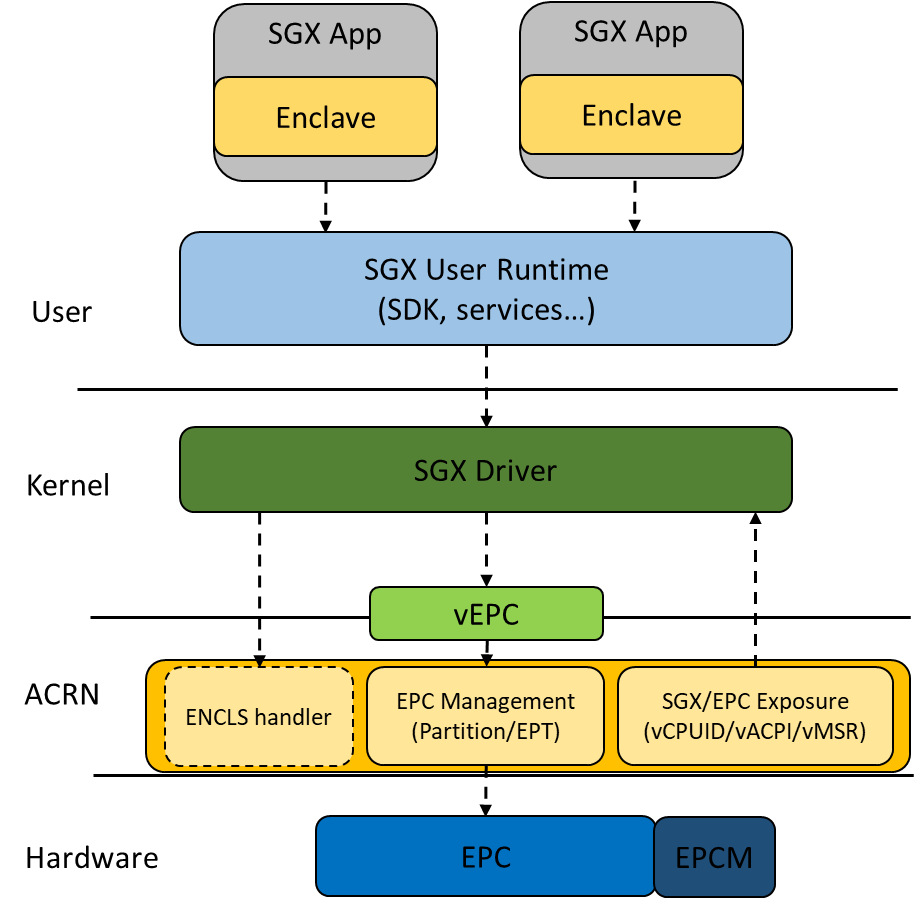
\includegraphics[width=0.4\linewidth]{pic/sgx.png}
        \caption{Intel SGX隔离机制}
        \label{sgx}
    \end{figure}


    同时Intel设计了一套用于检验硬件身份的协议,防止非SGX硬件平台伪造身份信息。该协议主要提供两种身份验证功能,分别是本地验证和远程验证。本地认证用于两个处于同一平台上的Enclave进行身份认证。具有SGX功能的CPU都有一个硬编码的加密密钥,只有Enclave能通过特定指令获取,因此处于同一平台的Enclave使用对称密钥进行消息的加解密处理即可认证身份信息。同一平台上的Enclave也可以使用该方法进行加密通信。远程认证是Enclave向远程的用户证明硬件身份信息。Enclave会将身份信息和平台信息等等进行封装,再通过一个特殊的Quoting Enclave进行本地验证后,将信息打包处理,最后使用Intel提供的Enhanced Privacy Identification方案进行签名,从而生成一份有效的身份证明。EPID签名方案是组签名,Intel无法得知该签名来自哪一个CPU,只能区分该CPU的组别,从而实现了隐私保护。远程的验证者向Intel Attestation Service服务提交获取的身份证明即可进行验证。



    SGX的核心原理是将应用程序在隔离的Enclave中运行,Enclave是一种可信执行环境,可以在普通的应用程序和操作系统之外运行。Enclave可以保证应用程序中的敏感数据和代码不会被未经授权的程序或系统访问。SGX的工作原理简单描述如下:
    \begin{itemize}
        \item 创建Enclave:应用程序通过调用API创建一个Enclave,这个Enclave是一个受保护的内存区域,只有Enclave内的代码可以访问它的数据。
        \item 加载代码和数据:应用程序将需要受保护的代码和数据加载到Enclave中。
        \item 运行代码:应用程序在Enclave中运行代码,Enclave会对代码的执行进行保护,确保不会被未经授权的程序或系统访问。
        \item 返回外部不可信区:Enclave执行代码完毕后,会通过接口反汇外部不可信区域,接下来操作系统会接管程序,可以再次进入Enclave或者销毁Enclave。
        \item 销毁Enclave:当应用程序不再需要Enclave时,可以通过调用API来销毁Enclave,这样Enclave中的数据和代码就会被清除。
    \end{itemize}

    \begin{figure}[H]
        \centering
        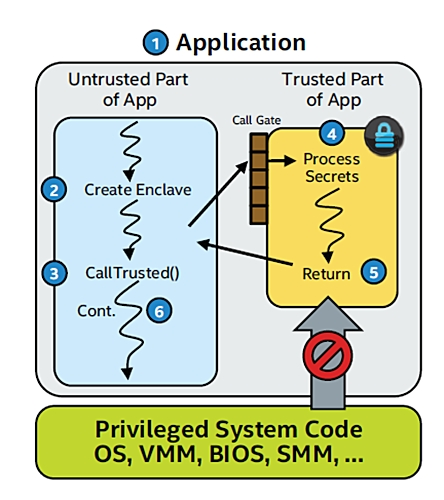
\includegraphics[width=0.4\linewidth]{pic/intelsgx.jpg}
        \caption{Intel SGX工作流程}
        \label{intelsgx}
    \end{figure}
    
    总的来说,SGX通过硬件隔离的方式保护应用程序的敏感数据和代码,这种隔离是软件无法实现的。通过SGX,应用程序可以在安全的环境中运行,即使操作系统或其他程序被攻击,应用程序中的数据也能得到保护。


    \section{SGX技术的应用}
        SGX技术所提供的隔离环境在隐私保护和机密计算等领域有巨大应用前景,许多现有的SGX应用主要服务于云计算,外包计算等场景。
        云计算相比本地搭建服务器而言,具有低成本,易于维护升级等优势,因此越来越多计算服务会将程序部署在云服务器上。
        云计算场景的安全性基于半诚实模型(敌手遵循协议规范,但可能试图从协议记录中了解更多允许的内容),出于利益和声誉等因素,服务商不会主动去攻击用户的云服务器。近年来,用户对于敏感信息的安全要求越来越高,当使用云服务器时,用户不得不考虑Ring0攻击者的威胁。例如云服务器上的数据库,若其中存储了涉及隐私的数据,拥有者并不希望非授权用户读取其中的内容。最简单的方法是通过加密来保护数据库内容,但是加密的方式效率低,会引入较大的计算开销,无法适应高速读写场景。
        SGX能够提供高效的隐私计算环境,为一些密码学瓶颈问题和隐私保护问题提供解决思路。例如,SGX本身具有的机密性和完整性保护能够很好地实现隐私计算和可验证计算,可以在区块链应用场景下发挥重要作用。

        \subsection{云计算}
        EnclaveDB\cite{priebe2018enclavedb}实现了一种基于内存的安全数据库,将数据库分为两个部分,如图\ref{enclavedb}所示,一部分是Enclave,另一部分为非Enclave的外界部分。该系统提出了安全假设,攻击者可以控制服务器的软件栈,但是不能控制Enclave中的代码。可信硬件的侧信道保护问题一直仍待解决,因此拒绝服务攻击和侧信道攻击不在考虑范围之内。所有的敏感数据,表,索引,查询,中间状态等等,都以内存数据的形式存储在Enclave中,由SGX技术提供机密性和完整性保护。如图所示,客户端会对Query进行预处理,防止服务器端对查询进行篡改。客户端将查询进行预编译并打包,将打包后的查询直接传输至Enclave。客户端会在传输的二进制数据中嵌入元数据,以防止任何服务器端对交互数据的破坏,实现完整性保护。用户会直接和EnclaveDB建立安全连接,生成一个共享会话密钥。在会话创建期间,用户通过Enclave生成一个密码学度量值,来验证身份信息。在后续交互过程中,用户和Enclave可以使用该密码来加解密信息,而服务器无法获得任何有用的信息。当数据库查询发生错误时,会抛出错误信息。错误信息也是一种服务器可以捕获的额外信息,为了防止泄露输入和输出,错误信息被分为两个种类,秘密相关错误和非秘密相关错误。秘密相关错误表示直接或间接和敏感信息相关的错误,比如表中的值。当执行引擎发生错误时,EnclaveDB会将错误信息转化为通用错误,并将错误代码和信息进行打包,加密后发送给用户。即使攻击者进行监听,也只会得知发生了错误,无法得知引发错误的具体原因。基于TPC-C压力测试实验,该方法在提供强安全性的情况下引入至多40\%的额外时间开销。由于云数据库所在的服务器端不受用户控制,攻击者可以切断平台的电源,给内存数据库造成巨大威胁,因此需要在额外的负载和数据可恢复性方面做出权衡。
        \begin{figure}[H]
            \centering
            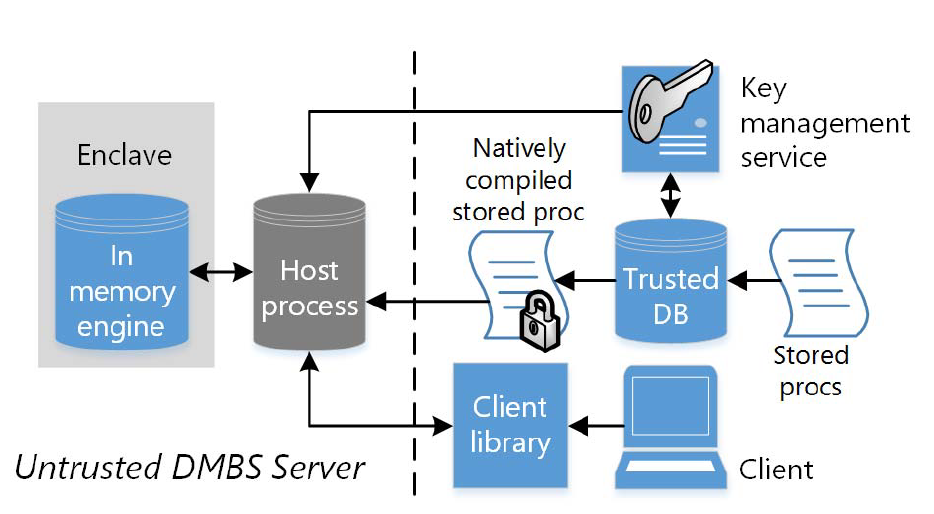
\includegraphics[width=0.7\linewidth]{pic/enclavedb.png}
            \caption{EnclaveDB整体设计架构}
            \label{enclavedb}
        \end{figure}
        
        % DelegaTEE\cite{matetic2018delegatee}实现了一种具有隐私保护的访问控制模型,能够允许用户灵活地将一系列服务提供商的凭据和权限委托给其他用户和第三方,在此过程中不会泄露用户的隐私数据。
        
        BITE\cite{matetic2019bite}提出了一种能够提供隐私保护的安全区块链数据库。该系统框架同样是将数据库放在外部存储中,而Enclave主要负责与用户交互和执行操作。虽然SGX为用户提供了代码执行过程的隐私性和完整性保护,但是磁盘不在SGX的安全模型中,直接使用Enclave去读取外部数据库仍然会泄漏用户的地址和交易。BITE使用了Path ORAM\cite{stefanov2018path}策略来读取外部数据库,可以混淆每次的外部读取操作。即使攻击者从操作系统层面来监视磁盘读取操作,但也无法得知Enclave具体读取了哪一块数据。区块链数据库很容易验证当前状态是否为最近更新的,用户只需要在其它节点下载当前最新的区块哈希,然后进行比对即可。当Enclave接受到用户的查询请求时,会通过Path ORAM策略扫描区块链数据库,当查询到某个块包含用户的交易时,就会在最后返回信息中包含该块,否则只包含该块的区块头信息。BITE对于Enclave也进行了侧信道攻击保护。对于时间侧信道攻击,比如说在只有出现包含对应地址的交易的时候,才会计算Merkel树路径,其他情况下不会存在hash计算,这是个非常典型的侧信道攻击,该系统采取的措施就是所有的扫描都要计算Merkel树路径。其次是针对控制流的侧信道攻击,为了进一步减轻不同路径的执行差异,该系统使用了一种指令层面的优化,就是使用cmov指令来消除循环。cmov指令的一个好处就是不论执不执行mov操作,只要是源操作数是内存地址,就一定会先读取出来。在拷贝区块链数据库内容时,采用了cmov指令,为了隐藏内存地址,将源来区块链的每个地址都条件写入目的地址,以实现消除差异。实验表明,BITE为轻型客户端提供了隐私保护,而不会影响完整节点的性能,经过修改后的区块链数据库只会引入大约4 GB的额外存储开销,每次客户端请求只需要12KB的通信开销。
        
        SCONE\cite{arnautov2016scone}实现了一种基于SGX技术的Linux安全容器,保护了容器内的数据不被具有更高权限的人员或者程序访问。因为往往在云服务器场景下,用户在容器中跑的服务通常都是像Apache、NGINX这样的只使用少量系统接口以及通过标准输入输出流或者套接字而不是直接访问其他 I/O 设备的服务,这刚好是适应了小 TCB 的场景。同时因为Enclave里的程序访问Enclave外的内存是没有额外性能开销的,基于硬件的实现也让Enclave内的程序运行速度与正常模式下几乎持平,只有内外数据交换会消耗少量CPU周期来完成。

        VC3\cite{schuster2015vc3}首次提出了允许用户在云中运行分布式 MapReduce 计算的框架,同时对用户的代码和数据保密,并确保正确性和结果的完整性。该框架下代码被分为两个部分,分别是$E^{+}$和$E^{-}$。其中$E^{-}$是需要被加密的代码,可以保护不被泄露。而$E^{+}$是公开的代码,主要实现密钥交换协议。通过密钥交换协议,Enclave可以得到远程用户的密钥,将该密钥用于解密E-部分的代码。整个过程将不可信的操作系统,管理员等等排除在外。


        \subsection{区块链}
        Cheng\cite{cheng2019ekiden}等提出一种基于可信执行环境的智能合约隐私计算平台Ekiden,能够对智能合约的输入,执行,输出均进行加密保护。如图\ref{ekiden},智能合约经过加密后存储在区块链上,用户需要调用合约时,首先通过加密信道传递程序参数,然后通过可信执行环境取回智能合约进行解密,并在其中完成执行过程,最后向用户返回进过加密的计算结果。该方案需要一个额外的分布式密钥管理中心,为该系统提供密钥管理功能。而该方案下的分布式密钥管理中心成员是固定的,无法动态加入和离开,属于一种中心化解决方案,导致该方案安全性仍然面临威胁。CONFIDE[7]在此基础上做出了改进,重新定义了一种智能合约编程模型,将智能合约分为公开部分和隐私部分,经过特定的编译器会将所有涉及隐私信息的数据标记为私有的。在智能合约执行过程中,公开部分的执行交给外部运行环境,而隐私部分的执行交给可信执行环境,避免了整个智能合约全部运行在可信执行环境中,提升了智能合约的执行效率。但是该方案将隐私数据的边界交由用户进行定义,极易导致差分攻击,给用户和代码审计人员带来困难。

        \begin{figure}[H]
            \centering
            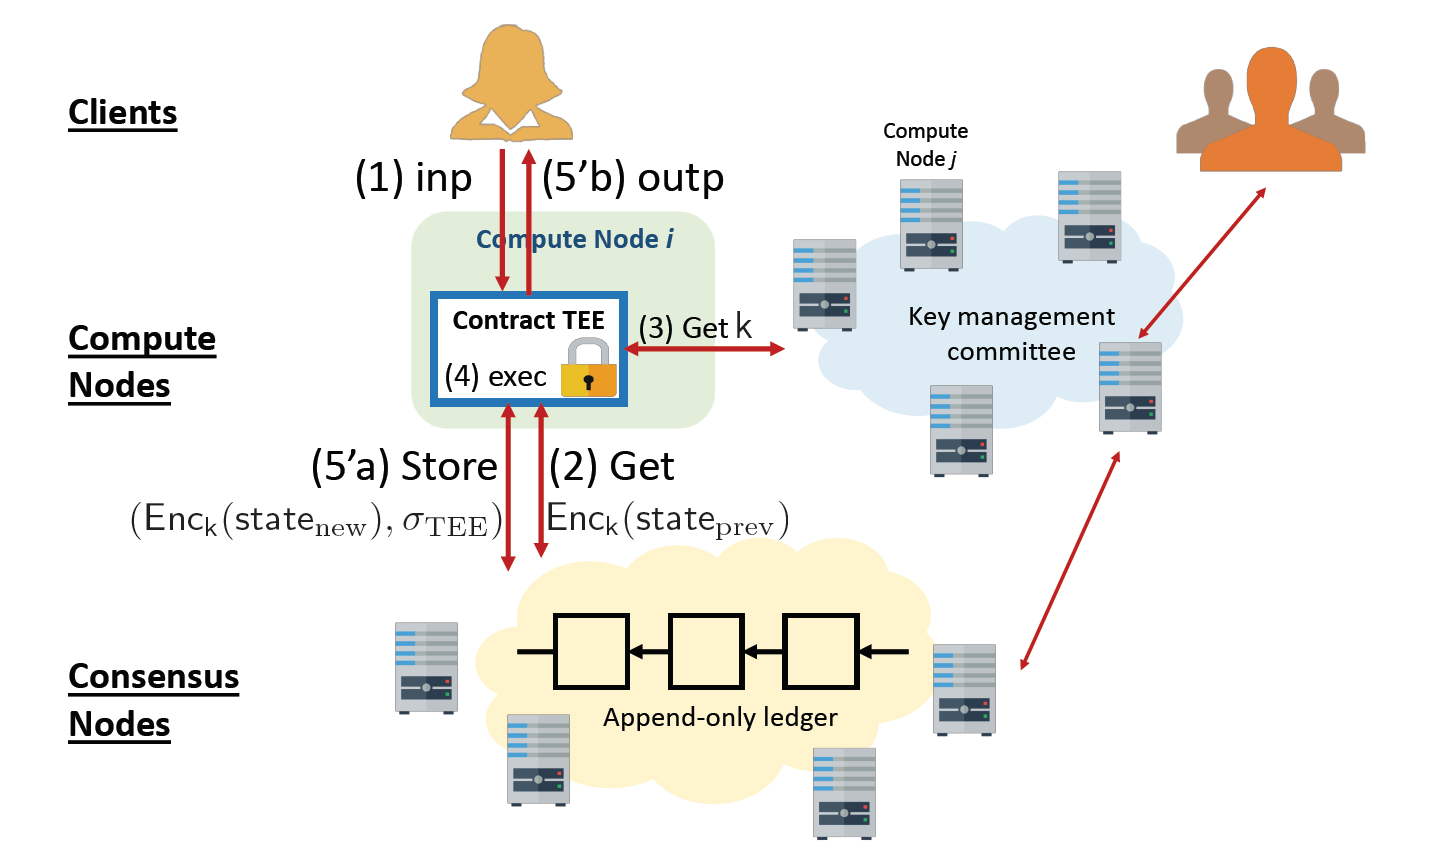
\includegraphics[width=0.7\linewidth]{pic/ekiden.png}
            \caption{Ekiden工作流程}
            \label{ekiden}
        \end{figure}


        FastKitten\cite{das2019fastkitten}基于可信执行环境提出了一种能够在比特币网络上运行的隐私智能合约模型。比特币没有提供图灵完备的虚拟机模型,因此比特币本身不支持智能合约。而现在的可编程加密货币(比如以太坊)存在速度慢、交易贵、运行时无隐私保护等问题。因此,FastKitten针对比特币网络提出了一个能够在链外执行(off-chain execution)且能执行多个轮回(multi-round)的高效的智能合约协议。该方案在TEE中实现了基于比特币的虚拟机模型,使用特定语言编写交易执行逻辑,同样达到了智能合约的功能,具有较强的隐私性和安全性以及执行速度快的特点。FastKitten测试的互动在线游戏,参与者之间有几毫秒的回合延迟。此外,FastKitten还讨论了许多可进行的扩展,如支持私有状态和安全输入,提升智能合约的机密性;支持可能跨越多种不同加密货币的合约,每个参与者可以使用个人喜欢的货币来处理合约中的资金。FastKitten与前述的Ekiden很类似,但FastKitten主要针对复杂的反应式多轮合约的链外执行,而Ekiden主要是为单轮合约执行设计的。
        
        总的来说,基于可信执行环境的隐私保护方案在实际应用中还存在许多不足。其一是开发语言受限,无法和现有的智能合约开发模型适配,存在一些应用的开发和迁移障碍。其二是安全问题,可信执行环境的安全性一定程度上依赖于硬件厂商,这仍然是该类方案未能有效解决的安全问题之一。

        \subsection{通用程序}

        许多需要安全执行环境的程序都可以移植到SGX当中,但是SGX技术不支持直接运行常规的二进制可执行文件。并且SGX应用的开发框架和普通程序不同,需要把代码划分成Enclave内外两个部分,因此SGX上的应用移植代价比较高。微软提出了一种移植方案 Haven\cite{baumann2015shielding} 来解决该问题。Haven架构如图\ref{haven}所示,该框架从上到下依次是,Application层,LibOS层,Shield层,uRTS层,kernel层。其中Application层,LibOS层,Shield层都在Enclave内部,软件只需要和LibOS交互,整个Enclave内部均被SGX保护。LibOS直接满足Application的操作需求,或者向外让Host OS完成具体需求,软件应用则不需要修改代码。因为SGX是基于指令集的保护技术,所以该框架能够尽可能少地带来额外时间开销。比如对于 SQL Server 应用,Haven只会引入13\%的性能损耗。尽管如此,Enclave仍然会有小部分的操作(如系统调用)需要与外界接触。此外,SGX还有一些细节限制:EPC大小有限(比如256M),页错误等异常需要由外界OS来处理,部分硬件指令Enclave内不能调用等等。由于Enclave与外界有交互,该框架也会面临被攻击的风险,比如侧信道攻击和代码重用攻击\cite{biondo2018guard}等等。

        \begin{figure}[H]
            \centering
            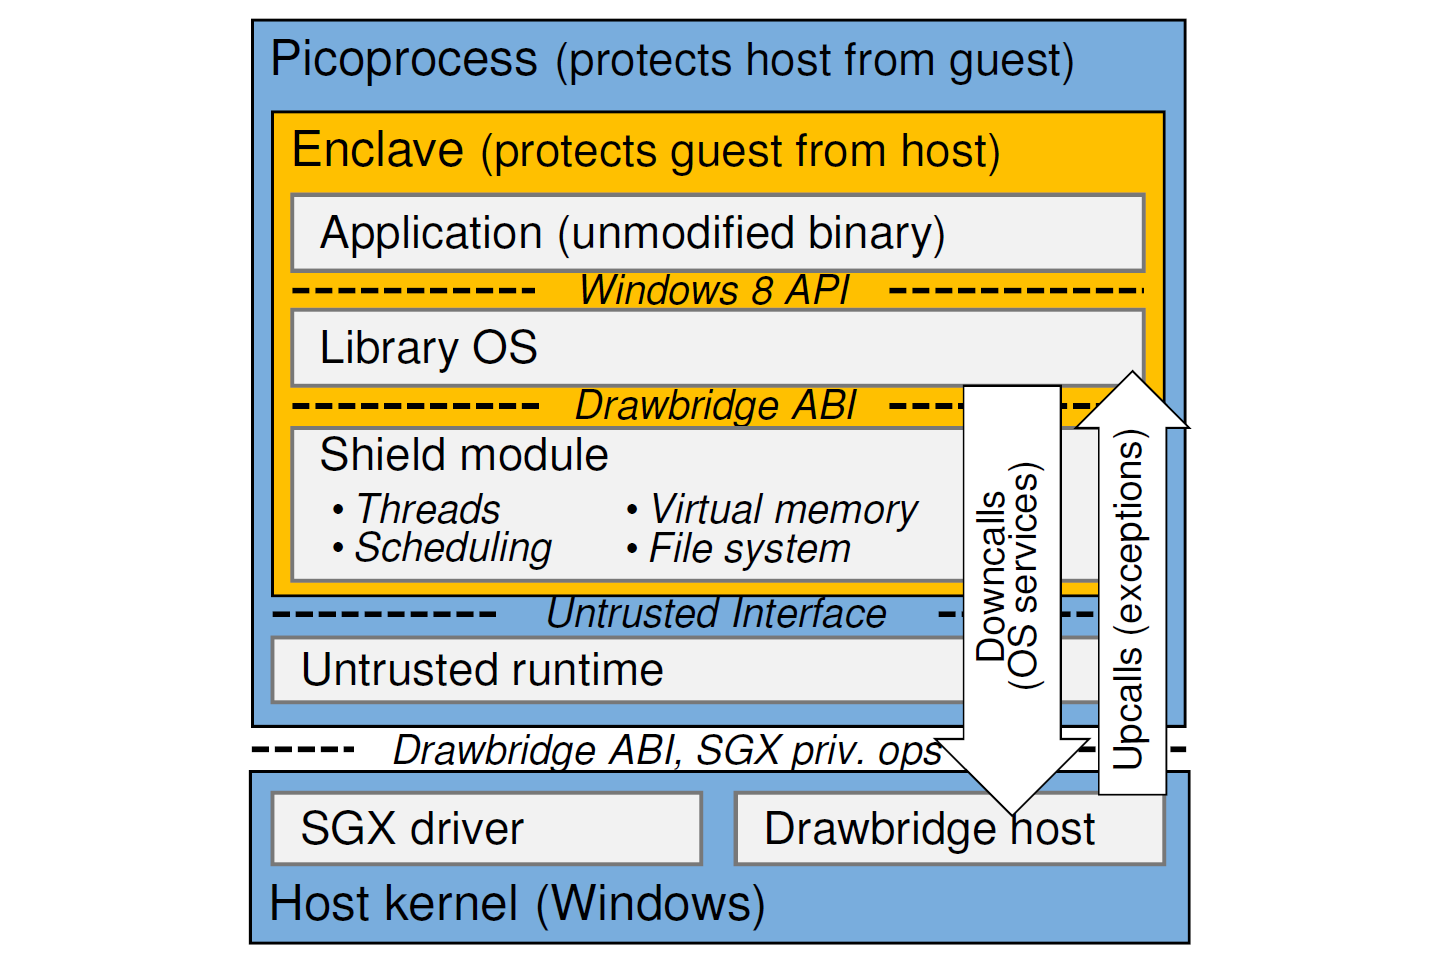
\includegraphics[width=0.7\linewidth]{pic/haven.png}
            \caption{Haven框架组成和接口}
            \label{haven}
        \end{figure}

        Graphene-SGX\cite{tsai2017graphene}和Haven类似,Haven是Windows下的实现,Graphene-SGX架构是Linux下的实现。Graphene-SGX框架的Enclave接口支持28个固定系统调用,其中18个系统调用会有检查。Graphene-SGX支持动态链接库和安全多进程,同时也允许一些未修改的软件直接运行,如 Apache,GCC,R interpreter 等等。

        \begin{figure}[H]
            \centering
            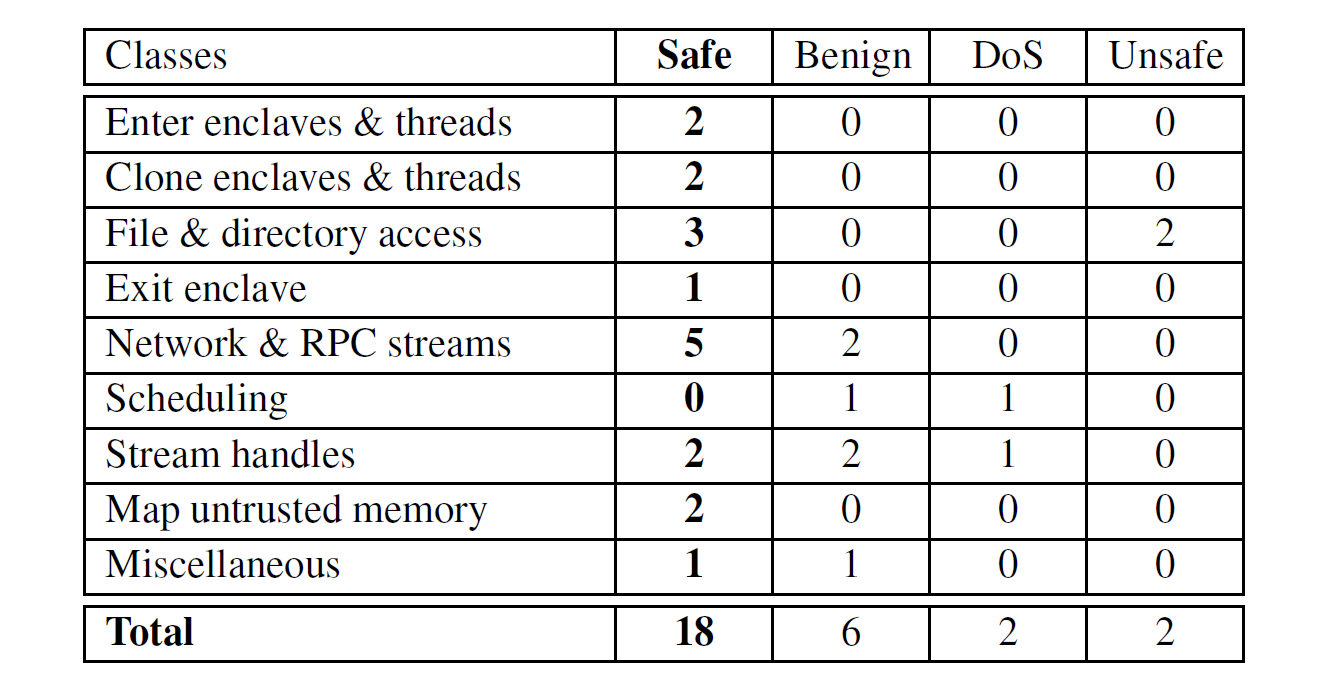
\includegraphics[width=0.7\linewidth]{pic/graphene.png}
            \caption{Graphene-SGX支持的18个系统调用}
            \label{graphene}
        \end{figure}

    \section{SGX安全问题}

        SGX无法抵抗软件层面的攻击,因为在Enclave内部运行的软件以及Intel SGX SDK都可能面临传统软件安全层面的威胁。因此在SGX中运行的程序需要进行严格的代码审计,避免因为程序自身漏洞(如栈溢出,内存泄漏等等)引发安全问题,给攻击者留下可乘之机。

        \subsection{SGX软件层面漏洞}

        代码重用攻击\cite{biondo2018guard}可以直接提取出SGX硬件编码密钥,从而破坏SGX中程序和代码的机密性和完整性。该攻击流程如图\ref{codereuse}所示,主要使用了ROP(return-oriented programming)攻击,通过特定的跳转代码,最终向内存中写入预先设计的shellcode来读取密钥并传输到用户空间。Enclave作为安全容器,通过特殊的通道和外界不可信操作系统进行交互。该攻击方式主要利用OCALL和Exception handling两种方式,将外界攻击者可以操控的数据带入Enclave中,而Enclave内部需要恢复处理前的寄存器状态,使得攻击者有可能操作寄存器,改变程序执行逻辑。该文中提出了ORET和CONT两种操作原语,能够循环调用特定的Gadget片段,进而向内存中写入恶意shellcode代码,改变原程序的执行逻辑。CONT原语可以控制CPU的通用寄存器,ORET原语可以控制rdi寄存器。因此CONT原语可以修改rip指向Gadget片段,修改rsp指向fake stack。CONT原语执行完毕后,rip会指向Gadget片段起始位置,而Gadget片段代码执行完毕后又返回到ORET原语。ORET原语修改rdi寄存器指向下一个构造的恶意CONT ctx结构体,最后再次返回到CONT原语。使用该攻击方法,攻击者只需要使用74字节长度的shellcode即可完成攻击。并且该攻击对敌手模型的要求较低,不需要依赖内核权限,只需要在用户态能够触发栈溢出漏洞即可。基于C/C++的大型软件中缓冲区溢出漏洞并不少见,攻击者只需要通过远程交互即可构造恶意输入触发缓冲区溢出漏洞,进而完成代码重用攻击。代码重用攻击是基于SGX SDK的攻击漏洞,因此影响力非常广泛,对SGX应用产生了巨大威胁。即使开启了代码地址空间随机化,但是SDK内部的代码并不会被随机化,所以无法有效抵御该攻击方法。出现该漏洞的原因在于SGX恢复上下文的时候没有实现原子性,被攻击者精心伪造的数据结构控制了恢复后的上下文。其中\cite{cui2021smashex,jang2017hacking}也是利用类似的机制缺陷实现了攻击。该文章提出了两种可能的防御机制。第一种是在上下文恢复的结构体中加入一个秘密值,每次对结构体的操作都需要检查该秘密值。该秘密值也是内存数据,如果攻击者能够通过额外的方式泄露该秘密值,那么就可以绕过该检查机制。第二种防御措施是为SGX SDK设计更细粒度的地址随机化机制,这样可以进一步加大攻击者发动ROP攻击的难度。

        \begin{figure}[H]
            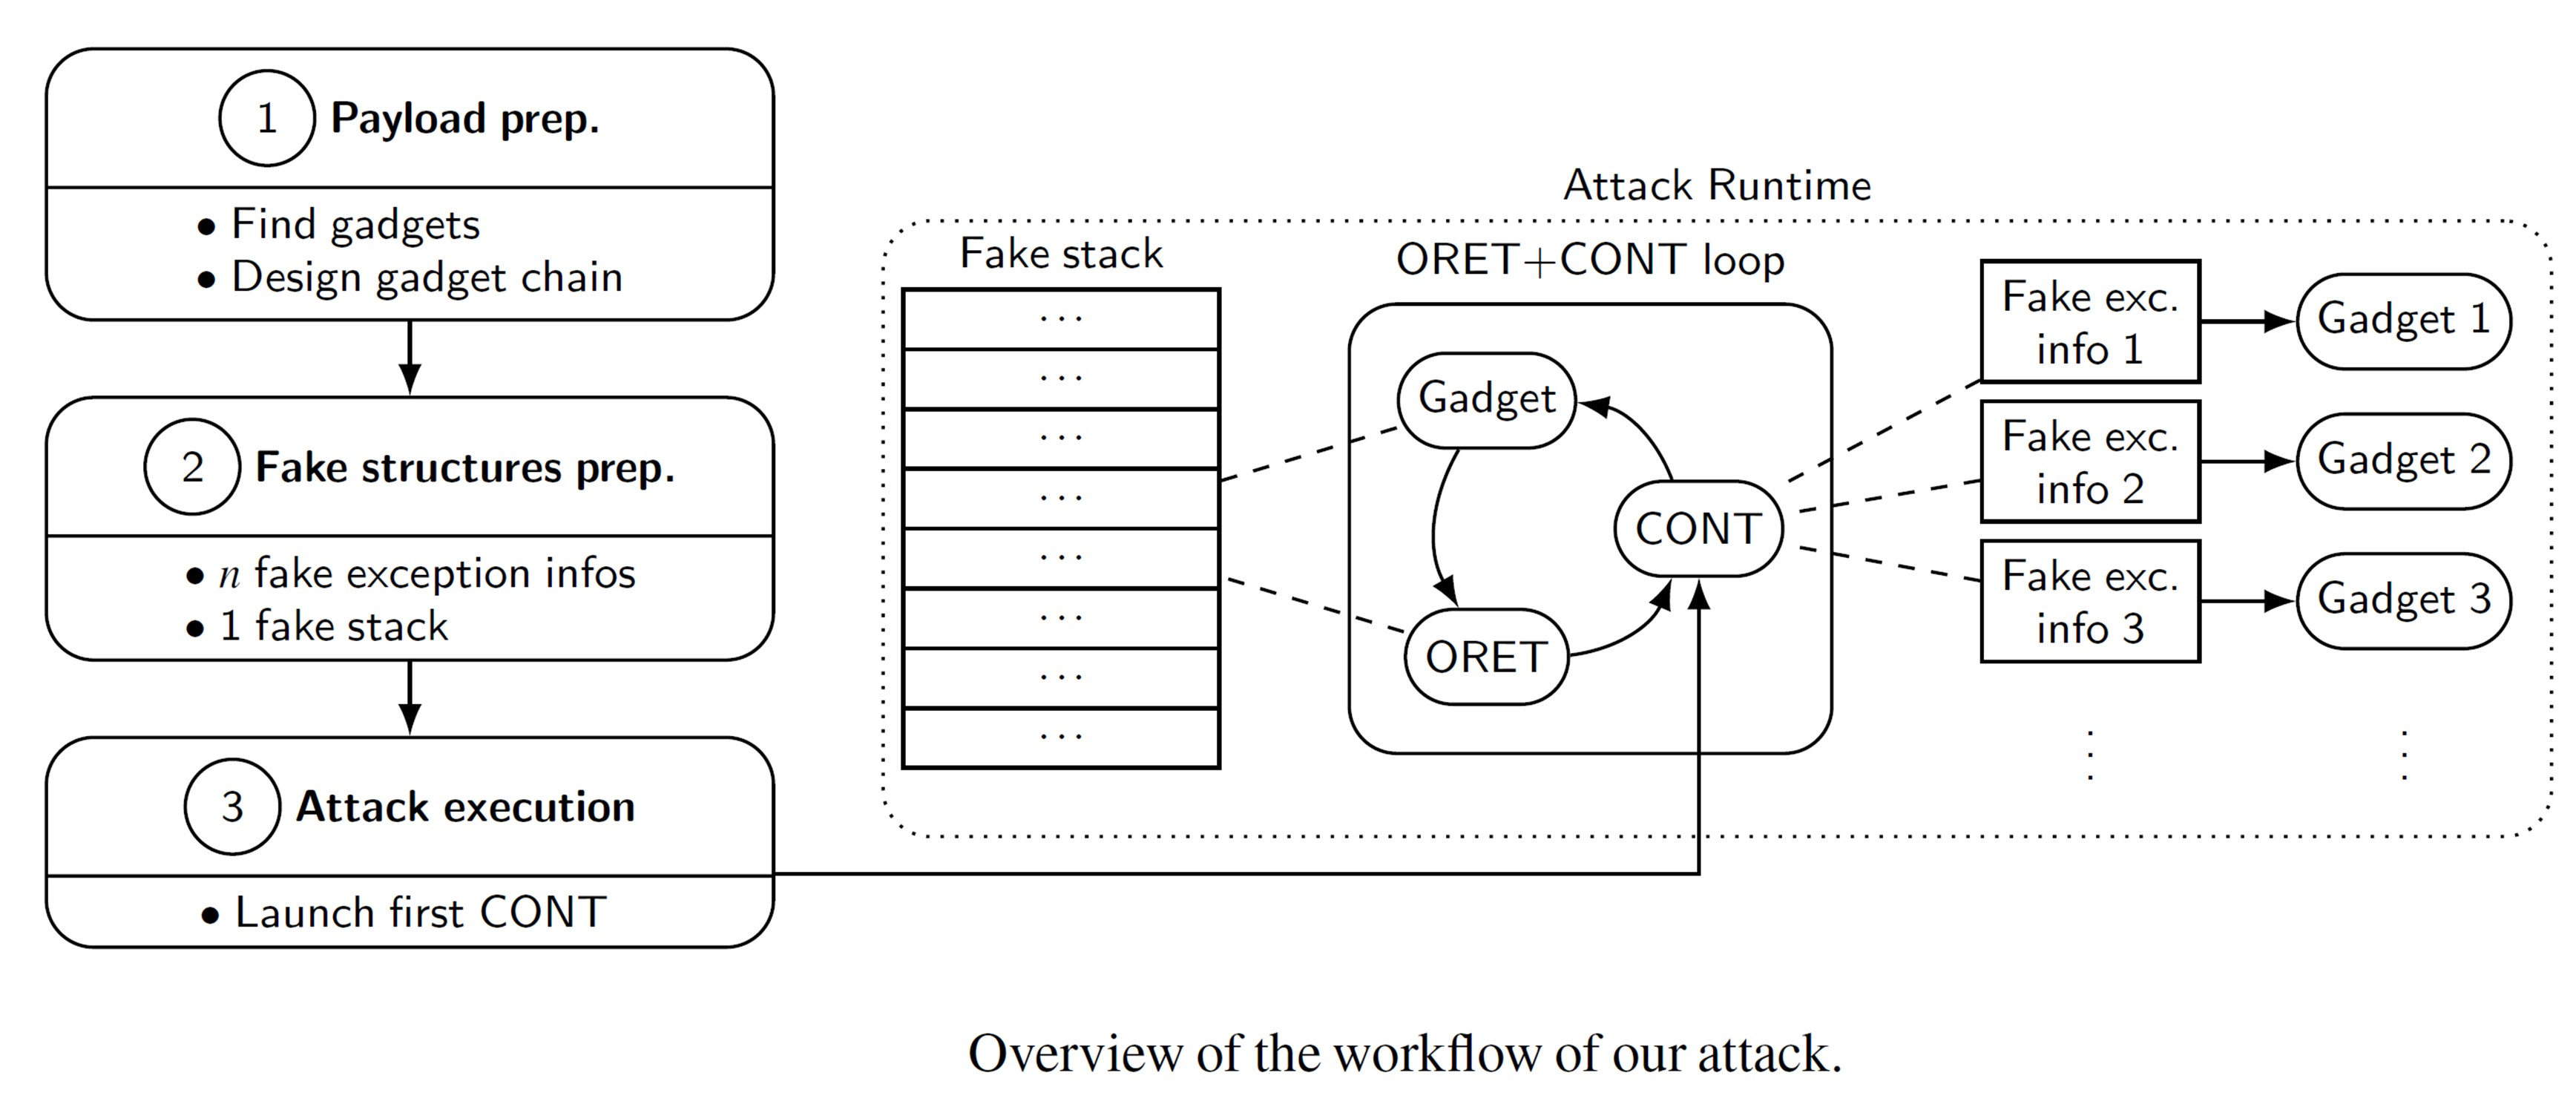
\includegraphics[width=1\linewidth]{pic/attack.jpg}
            \caption{code-reuse攻击流程图}
            \label{codereuse}
        \end{figure}

        \subsection{SGX安全防御方法}
        SGX为用户提供了安全的执行环境,但是SGX程序和普通可执行程序差距较大,使得SGX的编程模型变得尤其复杂,对开发者并不友好。Enclave内部不支持所有的操作系统级系统调用,需要当作外部不可信函数进行调用,并在EDL文件中进行声明。同时,Intel提供的SGX编译器edger8r只支持C/C++,并限制了部分C/C++的外部库功能,使得某些上层应用开发变得困难。尽管SGX能够保护重要应用程序的安全性,但是这些应用程序使用如C/C++等不安全的语言开发,仍然可能存在传统的内存安全漏洞,对SGX的安全模型带来威胁。
        
        针对该问题,百度安全实验室提出了一种基于Rust的SGX程序开发工具集Rust SGX SDK\cite{wang2019towards},它将Rust语言和Intel SGX技术进行结合,允许用户使用Rust语言开发SGX应用程序。
        Rust是一种系统级编程语言,由Mozilla开发。Rust旨在提供C++的性能和控制力,同时避免其常见的安全问题,例如缓冲区溢出、空指针引用和数据竞争。 Rust的设计目标是提供一种安全、并发和实用的编程语言,它在性能和可靠性方面都非常强大。Rust语言在许多领域都有应用,例如网络编程、系统编程、Web开发、机器学习等。得益于Rust语言的内存权限管理等优势,程序员可以基于该SDK开发出没有内存安全漏洞的Intel SGX可信程序,且性能几乎没有额外开销,因此Rust SGX SDK适合用于在SGX中开发大型的系统软件。

        SGX内部不提供系统调用,因此所有的系统调用被视为外部非安全区函数,需要借助SGX的OCALL操作来调用外部操作系统的系统调用函数。常规Rust编程模型下的std标准库实现是基于底层系统调用,因而无法直接在SGX开发环境下使用。Rust SGX SDK在Rust编程模型上进行了大量改写工作,重构了std标准库,并在此基础上开发了运行时库、密码组件库、底层通信库等等。如果通过Rust进行程序开发,只需要在普通的Rust源文件里开启no\_std属性,去掉所有和std相关的引用,并引入重构的std标准库即可在SGX环境下正常使用。Rust SGX SDK的高可移植性使得在SGX环境下开发大型应用成为可能。而Rust本身作为安全类型语言,为编程者提供了安全编程模型的同时也保证程序执行效率接近C/C++,成为SGX程序的可选开发语言之一。

        Asylo\cite{asylo}是Google的一个开源软件项目,其目的在于帮助开发者在云计算环境中编写安全的应用程序。Asylo提供了一个开发框架,使得应用程序可以在隔离的、可信的执行环境中运行,以提高应用程序的安全性。Asylo 支持多种安全执行环境,包括 SGX 和 TrustZone 等。Asylo 自身支持一些安全的编程接口和库,如加密算法库和身份验证库,以帮助开发者实现安全的应用程序。Google Asylo是基于Intel SGX PSW \& SDK封装形成的新的抽象。从实现代码可以分析得出Google Asylo在切换Enclave Mode和Normal Mode时,仍然使用了Intel SGX软件栈,包括由EDL文件形成的Trusted/Untrusted Stub,因此Google Asylo是位于Intel SGX PSW\&SDK的上层实现。

    \section{总结与展望}

        SGX技术的复杂性也增大了其攻击面,近年出现了越来越多针对SGX技术的攻击方法。SGX功能在最新的桌面端Intel CPU已经被移除,将会逐渐偏向于服务器端。在未来,SGX技术应该发展为大规模云服务,为用户提供各种定制的SGX应用。同时,SGX远程认证技术应该提供用户本地化功能,便于用户搭建本地SGX计算网络,避免使用IAS带来性能瓶颈。SGX2允许Quote验证行为交给第三方平台。第三方平台可以拉取Intel Attestation Service的证书缓存,用于验证Enclave生成的远程证明。每次用户和Enclave进行远程验证不再需要通过Intel Attestation Service,可以将该服务交给第三方平台进行实现。这对构建分布式应用非常有利,各个Enclave之间只需要和第三方平台进行交互。而第三方平台可以部署在本地,使得整个验证过程效率极大提升。同时,不依赖Intel Attestation Service保证了Intel无法介入后续验证过程,提高了系统整体的安全性。SGX2新增EDMM(Enclave Dynamic Memory Management)特性,支持动态调整Enclave所用物理内存。
        SGX2还支持EPC大内存,最高达1TB。SGX1中用于加密内存的Intel MEE被改为Intel TME。但Intel TME不再维护哈希树,即不提供完整性保护。

        SGX技术凭借自身的特性在安全领域发挥了重大作用,极大推动了可信计算领域的发展。其基于硬件的安全设计原理不仅实现了最小化安全假设,同时也保证了较小的额外开销。SGX在软件层面提供了许多可信计算的方案,但是也面临各类安全问题。未来,SGX技术需要更加精细化地定义安全界线和安全模型,以提高其安全性。
    
    \newpage
    \bibliographystyle{unsrt}
    \bibliography{ref}

\end{document}


